\section{Zielsetzung \& Anforderungen}

\subsection{GUI}

\begin{frame}{\insertsubsection}
    Grafisches Benutzerinterface für die UmachVM
    zur Entwicklung und für das Debuggen
\end{frame}

\subsection{Anforderungen}

\begin{frame}{\insertsubsection}
    \begin{itemize}
         \item Gui und Core eigene Prozesse
         \item Debugging
	 \begin{itemize}
             \item Setzen von Haltepunkten
             \item Einzelschritt
             \item Anzeigen der Codestelle
             \item Auslesen und Manipulieren der Register und Daten
         \end{itemize}
         \item Plattformunabhängig
    \end{itemize}
\end{frame}

\section{Debugging}

\subsection{Aufgaben eines Debuggers}

\begin{frame}{\insertsubsection}
    \begin{itemize}
         \item Steuerung des Programmablaufs (Haltepunkt, Einzelschritt)
         \item Inspizieren (Daten, Zustand)
         \item Modifizieren (Daten, Zustand)
    \end{itemize}
\end{frame}

\subsection{Realisierung der Steuerungsfunktionalität}

\begin{frame}{\insertsubsection}
    \begin{itemize}
         \item Temporäres ersetzen von Instruktionen durch spez. Interrupt
         \item Abgleich der Instruktionsadresse (Hardware, Software)
         \item Umach
         \begin{itemize}
             \item Abgleich der Adresse
             \item Assembler liefert Tabelle
         \end{itemize}     
    \end{itemize}
\end{frame}

\section{Prozesskommunikation}

\subsection{Übersicht}

\begin{frame}{\insertsubsection}
    \begin{itemize}
         \item VM läuft als eigener Prozess
         \item Kommunikation zur Steuerung und Datenaustausch
         \item Debugging
         \begin{itemize}
             \item Steuerung der VM
             \item Auslesen der VM
         \end{itemize}     
    \end{itemize}
\end{frame}

\subsection{Schaubild}

\begin{frame}{\insertsubsection}
    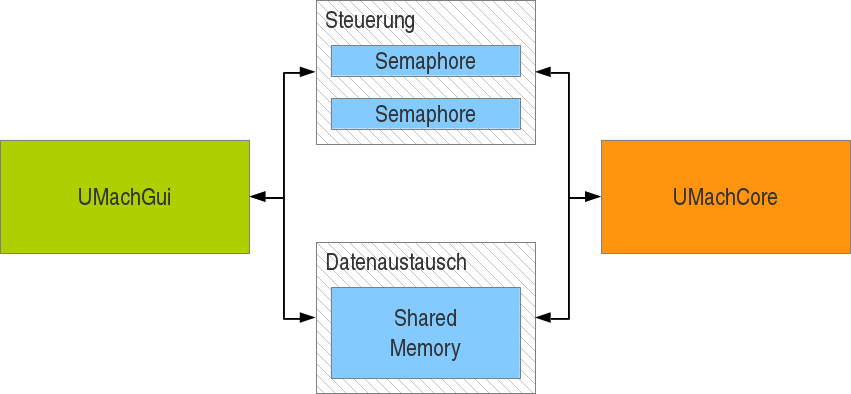
\includegraphics[width=\textwidth]{g1}
\end{frame}

\subsection{QSystemSemaphore}

\begin{frame}{\insertsubsection}
    \begin{itemize}
         \item Ressourcenzähler
         \item aquire()\\
         Ressource anfordern
         \item release()\\
         Ressource freigeben
         \item Blockiert Prozess wenn keine Ressource verfügbar
         \item Zugriff über ID
    \end{itemize}
\end{frame}

\subsection{QSharedMemory}

\begin{frame}{\insertsubsection}
    \begin{itemize}
         \item Prozessübergreifender Speicher
         \item Erster Konstruktoraufruf erzeugt Shared Memory
         \item Zugriff über ID
         \item attach()\\
         Anhängen an den Prozess
         \item detach()\\
         Abhängen vom Prozess
         \item Letzter Aufruf von detach() zerstört QSharedMemory
         \item Sicherstellung der Freigabe
    \end{itemize}
\end{frame}

\subsection{Kontrollzyklus}
\begin{frame}{\insertsubsection}
    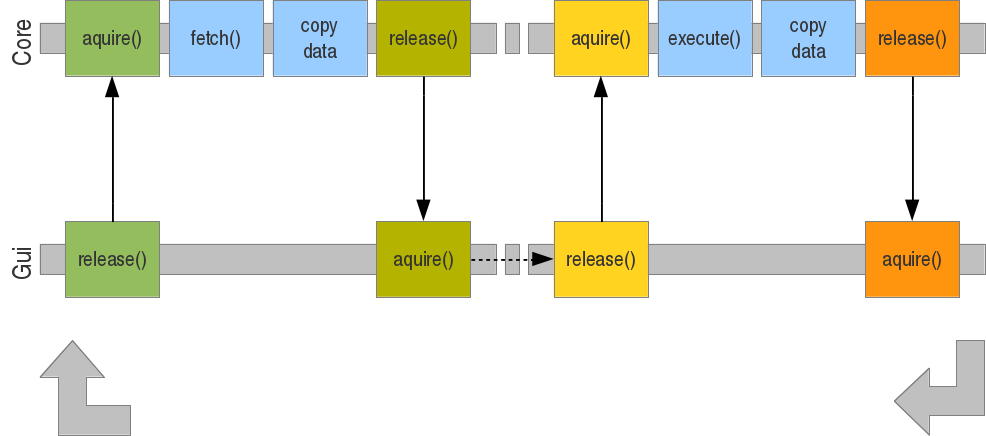
\includegraphics[width=\textwidth]{g2}
\end{frame}

\section{QT Bibliothek}

\subsection{Warum QT?}

\begin{frame}{\insertsubsection}
    \begin{itemize}
         \item Einfach zu verwenden, gute Dokumentation
         \item Plattformunabhängigkeit
         \item Flache Hierarchie - Einfach zu erweitern
         \item Vorhandene Erfahrungswerte
    \end{itemize}
\end{frame}

\subsection{Signal \& Slot Prinzip}

\begin{frame}{\insertsubsection}
    \begin{itemize}
         \item Alternative zu Callback
         \item Einfache Syntax
         \item Minimal langsamer als Callback
         \item Benötigt Meta Object Compiler
    \end{itemize}
\end{frame}

\subsection{Signal}

\begin{frame}[fragile]{\insertsubsection}
	\lstinputlisting[language=C++]{./Debugger/c2_signal.cpp}
\end{frame}

\subsection{Emit}

\begin{frame}[fragile]{\insertsubsection}
	\lstinputlisting[language=C++]{./Debugger/c2_emit.cpp}
\end{frame}

\subsection{Slot}

\begin{frame}[fragile]{\insertsubsection}
	\lstinputlisting[language=C++]{./Debugger/c2_slot.cpp}
\end{frame}

\subsection{Connect}

\begin{frame}[fragile]{\insertsubsection}
	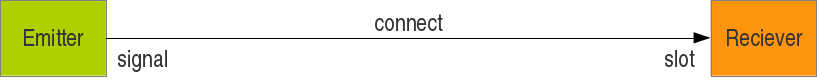
\includegraphics[width=\textwidth]{g4}
	\lstinputlisting[language=C++]{./Debugger/c2_connect.cpp}
	\lstinputlisting[language=C++]{./Debugger/c1.cpp}
\end{frame}

\section{GUI \& Demo}

\subsection{Projektdatei}

\begin{frame}{\insertsubsection}
    \begin{itemize}
         \item Projektdatei .umproject
         \begin{itemize}
         	\item Zugehörige Assemblerdateien
			\item Speicherung von Einstellungen und Haltepunkten
    	 \end{itemize}
         \item Benötigt Make-Routine
    \end{itemize}
\end{frame}

\subsection{Demo}

\begin{frame}{\insertsubsection}
    \begin{itemize}
    \item fibonacci.umx
    \item Haltepunkte
    \item Nächste Instruktion
    \item Registerinhalt
    \end{itemize}
\end{frame}

\subsection{Ausblick}

\begin{frame}{\insertsubsection}
    \begin{itemize}
    \item Speichern von Optionen
    \item Symbolinformation
    \item Manipulation Daten \& Zustand
    \item Weitere Ideen
    \begin{itemize}
    	\item Speicheranzeige
    	\item Graphische Darstellung Speicherbelegung
    	\item ...
    \end{itemize}
    \end{itemize}
\end{frame}
